\documentclass[12pt,twoside]{article}

\usepackage{graphicx}
\usepackage{fullpage}
\usepackage{subfig}

\graphicspath{ {figures/} }

\usepackage{etoolbox}
\patchcmd{\thebibliography}{\section*{\refname}}{}{}{}
\newcommand\tab[1][1cm]{\hspace*{#1}}

\begin{document}

\begin{titlepage}
	\begin{center}
		\vspace*{1cm}
		
		\Huge
		\textbf{Detecting Spoofed IP Packets Using TTL Analysis}
		
		\vspace{0.5cm}
		\LARGE
		
		\vspace{1.5cm}
		
		\textbf{Joseph Faulls\\}
		\Large
		ID: 1447637
		\vfill
		
		\LARGE
		MSci Computer Science
		
		\vspace{0.8cm}
		
		
\includegraphics[width=0.4\textwidth]{university_logo}
		
		\Large
		School of Computer Science\\
		University of Birmingham\\
		Supervised by Dr Ian Batten\\
		6th April 2018
		
	\end{center}
\end{titlepage}

\thispagestyle{plain}

\begin{center}
	\Large
	\textbf{Detecting Spoofed IP Packets Using TTL Analysis}
	
	\vspace{0.4cm}
	\large
	
	\vspace{0.4cm}
	\textbf{Joseph Faulls}
	
	\vspace{0.9cm}
	\textbf{Abstract}
\end{center}

% (1) it states the problem that you set out to solve, 
% (2) it describes your solution and method, 
% (3) it states a conclusion about the success of the solution. Be straightforward and factual and avoid vague statements, confusing details and "hype". Do not be tempted to use acronyms or jargon to keep within the half-page limit.

At the core of the Internet Protocol lies the datagram, small packets of information that provide a connectionless communication service across the Internet. These packets contain data such as the sender and receiver's IP address. However, to ensure a quick and connectionless protocol, this information is never validated. This can be exploited and the source IP address forged to any desired. This is known as IP spoofing. The motives to fake a source address are almost exclusively malicious; for example, to conceal the origin of a cyber attack. 

Buried in the data of all IP packets is a value named 'TTL', or 'Time To Live'. This can be thought of as the lifetime of the packet. It exists to prevent data circulating a network or computer indefinitely. The lower this value is upon arrival, the further the packet has travelled. Therefore, we can infer approximately how far away the true sender is. If a packet arrives with a TTL value different enough from what is expected, given the IP address, we can deduce that the packet has taken a very different route. Consequently, the IP packet is probably spoofed.

This paper discusses the design and implementation of a tool to handle large volumes of data at high load, making decisions of whether any IP packets are spoofed based on the source address and TTL value. Discussions are mainly focused on the engineering challenges involved. The end product is proven to be sufficiently fast at handling very large amounts of data and acting reasonably quickly to block or limit potentially spoofed IP packets. The spoof detection rate of the tool is found to be over 90\%.

\vspace{2.5cm}

\begin{center}
	\textbf{Git Repository} \\
All code, test results, and generated statistics can be found at \\ \texttt{https://git.cs.bham.ac.uk/jxf438/final\_year\_project\_masters}
\vspace{2.5cm}
\end{center}

\newpage
\begin{center}
	\textbf{Acknowledgments}
\end{center}
%I cannot take all the credit for this glorious masterpiece of scientific pioneering. These bois helped too:\\
%Charlie Street for pointing out how much of a cretin I am at programming in C.\\
%Ian Batten for giving me the idea, pointing me in the right directions, answering my questions and prolonged stories about things he has in his loft.\\
%Jack Utterly for not getting pissed off at me when I crashed the school's PC for 100th time.\\
%Rachel Szpara for both guilting me and giving me dat sweet ass to motivate me.
It is only fair and deserving that I give thanks to all those who have given me continual help and support throughout this project. Without it, the journey would have been a grueling struggle and the end product lacking in substance.

Most of all I'd like to thank my supervisor, Ian Batten. Firstly, for the foundation of the project idea. But more importantly, thank you for reminding my why I chose to study computer science. Your enthusiasm and bountiful pool of (mostly useful) knowledge has made me more interested in this field more than ever - even to the point of considering a career in networking!

Secondly, I'd like to thank the School of Computer Science for it's constant support of supplying me with useful resources. In particular, I owe a great deal to Jack Utterly, who set up and maintained a SoCS machine to collect data. I am sorry for all the times you had to traipse down to reset the machine when I crashed it!

Thank you to all my computer science friends, whom made the 4 year journey so much more enjoyable and easier. In particular, Charlie - a simple thank you is not merely enough for the gratitude I have for the countless bugging and questions I've asked you. Heaven knows how much of this degree I owe you.

Lastly, thank you Rachel. Your diligence in your work has inspired me more than you know. This dissertation is undeniably better through the motivation you've given me.
\newpage
\tableofcontents

\newpage
\section{Introduction}
The information contained in the header of an IP packet is fundamental to the protocol. This data is the only way of knowing how to process the packet. Among the required information that all datagrams must contain, is a source address, destination address and a lifetime \cite{rfc791}.

% Without it, routers would not know where to send it, the receiver wouldn't know where it came from or what protocol it is using, and packets could endlessly circulate the Internet. 

Although, because datagrams are connectionless, there is no way to validate the correctness of these fields just by looking at the header. Faking the source address of a packet is known as IP Spoofing, and is already a well established problem \cite{ipSpoofIntro}\cite{ipSpoofing}\cite{spoofProblemStatement}. This can be achieved very easily through the use of off-the-shelf programs such as {\it hping} \cite{hping}, where faked packets can be forged in a single line command.

%change this first se
The motives to spoof an IP packet are almost exclusively malicious. The primary reason would be to conceal the origin of an attack - seeing as most systems keep logs of their Internet activity and IP addresses can be traced back to their physical location. However, this goes much further than just simply masking identity; many serious attacks rely on IP Spoofing. Some examples of these are described in section \ref{attacks}.

The most serious and widely used of these are a variety of denial-of-service attacks (DoS). The prime objective of these attacks is to exhaust the host's network resources such that it is unable to service legitimate requests. With the increase in availability of services that rent large networks capable of performing powerful DoS attacks, of those being monitored by Kaspersky Lab, a multinational cybersecurity company, the number of DoS attacks identified from 1st July to 30th September 2017 ranged from 296 and 1508 per day \cite{q3ddos}. Any business that offers online services is a target for these attacks and can cost a company anywhere from \pounds10,000 to \pounds1.68 million per incident \cite{ddoscost}.

Efforts have already been made to combat IP Spoofing to some degree of success. However, many of the techniques are intricate, costly to implement or have been made no longer possible. These are outlined in section \ref{defences}. 

It was mentioned that IP headers must include a lifetime, known as Time To Live (TTL). This is represented as an 8-bit decrementing counter of how many times the packet has hopped between routers. Upon reaching 0, the data is discarded. TTLs exists to prevent data circulating a network or computer indefinitely. 

Based on the assumption that the route taken by separate requests from the same source are very similar, or even the same, we can expect similar TTL values from a given source throughout all requests. Therefore, if a packet arrives with a TTL value statistically different enough from the expected one, we can assume that the packet has taken a very different route to get there. Consequently, the source address was probably spoofed.

However, different protocols use different initial TTL values. So simply comparing TTLs is not a viable option. Thankfully, the set of default TTL values for protocols is small. In almost all cases, default values are very commonly either 64 and 128 for TCP/UDP, or 128 and 255 for ICMP (Internet Control Message Protocol). Knowing this, we could make accurate, educated guesses as to what the initial TTL value was set to and therefore infer a 'hop-count'. For example, if we observe the following closely grouped data from a given source address: \texttt{4x57, 8x58, 10x121, 23x122}, we can assume the values in the high 50's had an initial TTL of 64, whilst low 120's started at 128. This means that packets took 6-7 hops in all cases. 

The problem now lies in calculating expected Time To Live values for every IP address. One approach would be to send a small echo request to the apparent source address and compare the TTL of the response to that of the request. However, there is a penalty associated for doing so. Whether this is too costly depends on the computing power capabilities and size of input stream.

More intuitively, we can log all the source addresses and TTL values for all incoming packets. Over time, a large database or map can be generated with expected values for all seen IP addresses. Then, when a request comes in, it's TTL is compared to ones seen before from that address.

The main limitation to this method is clear, what is to be done with an unseen address? A simple one-to-on mapping of IP addresses to expected hop-count might be too specific. It cannot be assumed that malicious traffic would contain a spoofed source address that has been previously seen by the server. Therefore, a mechanism to predict or calculate an expected hop-count value for unseen source addresses is required. 

Using TTL as an indicator to whether a given packet is spoofed is not an entirely novel concept. There have been two papers published discussing the plausibility of such an approach, both concluding it is not only possible, but viable. This paper explores an actual implementation of the theory, as well as analysis of data to validate if the assumptions made in the published papers 16 years ago are still valid today.

The worked carried out described in this paper can be split into three parts: the data collection tool in section \ref{kernel_tool}; the packet analysis and response tool in section \ref{analysis_tool}; and data analysis carried out to measure this method's theoretical effectiveness in section \ref{analysis}.

Whether due to limited resources, insufficient time frame or simply out the scope of this project, there are features that should be modified or added in order to make this method as effective as possible. These are outlined in section \ref{future}
%%%%%%%%%%%%%%%%%%%%%%%%%%%%%%%%%%%%%%%%%%%%%%%%%%%%%%%%%%%%%%%%%%%%%%
\section{Attacks Using IP Spoofing} \label{attacks}

Being able to fake the source of IP packets not only conceals the attacker, alleviating risk of being caught, but also plays a fundamental role in enabling a wide array cyber-attacks. Several of these methods will be explored into some depth to demonstrate how they could all be avoided if spoofed IP addresses could be identified and discarded.

One attack not strictly related to IP spoofing, but worth mentioning, is an IP or network routing attack. This is where a router makes false claims about itself to have traffic diverted towards it, usually for some malicious purpose such as monitoring traffic. Perhaps it claims to have direct links with far away routers, making it a preferred choice. This ultimately changes the route (thus, the average TTL) and allows passive spoofed packet detection using TTL to also act as a routing change detector. 

%%%%%%%%%%%%%%%%%%%%%%%%%%%%%%%%%%%%%%%%%%%%%%%%%%%%%%%%%%%%%%%%%%%%%%
\subsection{SYN Flood}
First discovered in 1996, the TCP SYN flood is a notorious and common method of a denial-of-service (DoS) attack \cite{rfc4987}. As with all DoS attacks, the aim is to stop the victim being able to respond to legitimate traffic. This is accomplished by taking advantage of the three-way handshake, the TCP connection establishment process (see figure \ref{figure_handshake}).

\begin{figure}[h]
	\begin{center}
		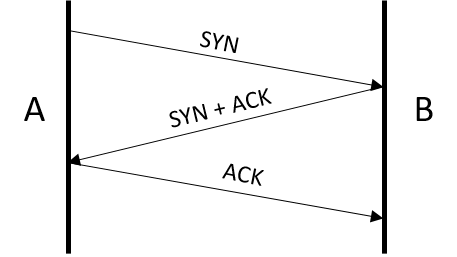
\includegraphics[width=4.57cm, height=2.57cm]{figures/three-way-handshake}
	\end{center}
	\caption{TCP three-way-handshake}
	\label{figure_handshake} 
\end{figure}

After receiving the first SYN request, the host B sends back the SYN+ACK packet and enters into a listening state, waiting for the final ACK. If the initial SYN request had a spoofed source address, this packet would be sent to a different machine than the one that started the handshake. Therefore, the host B will never receive the final acknowledgment packet and just keep waiting until a timeout. 

Although the data structure to hold the current state is relatively small, this soon adds up as more half-open connections are created, eventually causing the server to be unable to accept any more requests - denying legitimate users.

%%%%%%%%%%%%%%%%%%%%%%%%%%%%%%%%%%%%%%%%%%%%%%%%%%%%%%%%%%%%%%%%%%%%%%
\subsection{TCP Session Hijack} \label{hijack}
Interrupting and exploiting a valid computer session to pose as the trusted client is known as session hijacking. The TCP protocol makes this difficult to do by generating an initial sequence number (ISN). For a connection to be established, both parties must synchronise on each others ISN, and reply packets must include the ISN of the preceeding packet \cite{rfc793}. 

Therefore, for an attacker to hijack the session between a server and a host, impersonating the host, they must first acquire the sequence number and then ensure the server receives their reply packets before the host's. The latter of this can be accomplished via a denial-of-service attack targeting the host.

The job of acquiring the ISN is more challenging. If the attacker were on the same segment as the victim, this is a trivial job accomplished by sniffing packets. However, without access to the network traffic, the attacker must predict the sequence number. This can be done by exploiting the generation process or performing an rsh server attack \cite{tcphijacking}.

Even if the attacker goes through the trouble of acquiring the ISN one way or another, the requests to the server must be spoofed to pose as the victim and the average TTL will suddenly change. If this sudden change in TTL can be identified, the connection can be shut down and this attack can be nullified completely.

This is a unique attack in the fact it uses IP spoofing with TCP rather than the more attractive connectionless UDP packets. Techniques have already been developed to combat this with high degree of success. Network level hijacks can be prevented by encrypting the packets using any of the widely available protocols such as SSL or SSH.

%%%%%%%%%%%%%%%%%%%%%%%%%%%%%%%%%%%%%%%%%%%%%%%%%%%%%%%%%%%%%%%%%%%%%%
\subsection{Reflective UDP Amplification}
denial-of-service attacks often employ reflective UDP amplification to disrupt networks and systems. This technique allows for an attacker to amplify the malicious traffic using a third party server, whilst concealing the source of the attack.

Targeted servers, used to amplify the traffic, can either be rented or targeted. Typical servers used are ones with running applications that use connectionless protocols (like DNS or SNMP) and do not require authentication from their clients. Using multiple servers is desirable so that the malicious packets arrive from distributed sources. This means the victim cannot block all attack packets by blocking one server.

To get traffic to arrive at the victim, UDP request packets are sent to a server with the source address spoofed to be that of the victims. Therefore, the victim receives the reply packets, perhaps many times bigger than the small request packet sent. This means that the attacker can generate attack flows of many tens of Gb/s whilst only sending 1 Gb/s of traffic themselves.

\begin{figure}[h]
	\begin{center}
		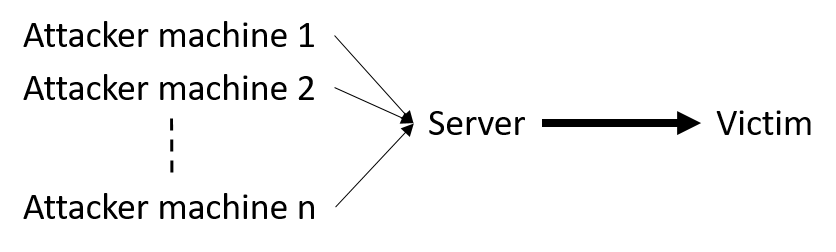
\includegraphics[width=8.36cm, height=2.52cm]{figures/udp-amplification}
	\end{center}
	\caption{Reflective UDP Amplification}
	\label{figure_amplification} 
\end{figure}

Due to the effective and highly accessibly nature of the attack, US-CERT (United States Computer Emergency Readiness Team) issued an alert on UDP-based amplification attacks in 2014 \cite{USCERT}.
%%%%%%%%%%%%%%%%%%%%%%%%%%%%%%%%%%%%%%%%%%%%%%%%%%%%%%%%%%%%%%%%%%%%%%
\subsection{Smurf Attack}

This is distributed denial-of-service attack (or DDoS - meaning the abusive traffic arrives from many different computers at the same time), in which the spoofed IP address is that of the victim's. Large numbers of Internet Control Message Protocol (ICMP) packets with the victim's source address are broadcast to computer network using an IP broadcast address \cite{rfc919}. Every machine on the network will attempt to send a reply to the source address, thus flooding the victim with traffic \cite{smurf}. 

\begin{figure}[h]
	\begin{center}
		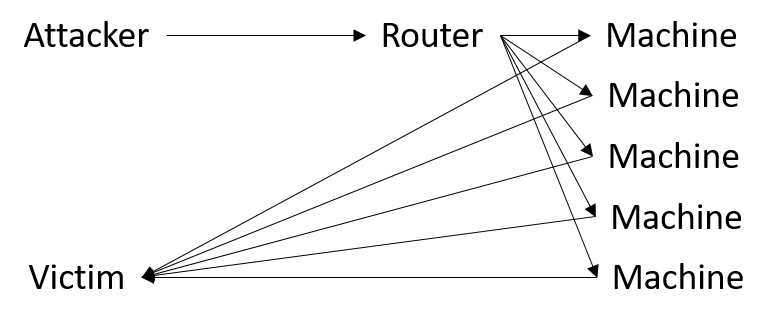
\includegraphics[width=7.67cm, height=3.22cm]{figures/smurf}
	\end{center}
	\caption{Smurf Attack: how one request can lead to hundreds}
	\label{figure_smurf} 
\end{figure}

\section{Related Work} \label{defences}
Efforts to prevent spoofed IP packets from being processed and regarded as legitimate can be categorised into active and passive methods. Both methods can either be implemented on a router or host level. 

Active methods attempt to verify the legitimacy of the source address by either tracing the packet, or detecting whether the supposed source was able to originate where it physically arrived from. However, passive methods simply classify a packet as being legitimate or not, and do not verify the actual source so cannot be used to establish accountability for attacks. The majority of work done to identify spoofed packets are active methods.

%%%%%%%%%%%%%%%%%%%%%%%%%%%%%%%%%%%%%%%%%%%%%%%%%%%%%%%%%%%%%%%%%%%%%%
\subsection{Eliminating Spoofed Packets from the Internet \cite{eliminating}}
Published in 2007 by the IETF Trust, this approach was motivated by the Source Address Verification Architecture Problem \cite{spoofProblemStatement}, a formalisation of the IP spoofing problem. Implemented at a router level, this method attempts to detect and discard any datagrams with spoofed addresses by devices that have an authoritative mapping between IP addresses and the network topology. Discarding spoofed packets at the earliest stage possible prevents any from circulating the Internet, nullifying any need to analyse packets at a host level.

A device that is close enough to the source to have a table between layer 2 (Data link layer) and IP addresses can discard any packets in which the IP address is not associated with (and is therefore assumed to be spoofed) the layer 2 address in the datagram. This device can be a CPE router (Customer Premise Equipment), ISP PE router (Premise Edge, meaning a router between one network service provider's area to outside their premise), NNI router (Network-to-network router providing interconnections of provider's networks), network switch or a host (see figure \ref{figure_eliminating}).

\begin{figure}[h]
	\begin{center}
		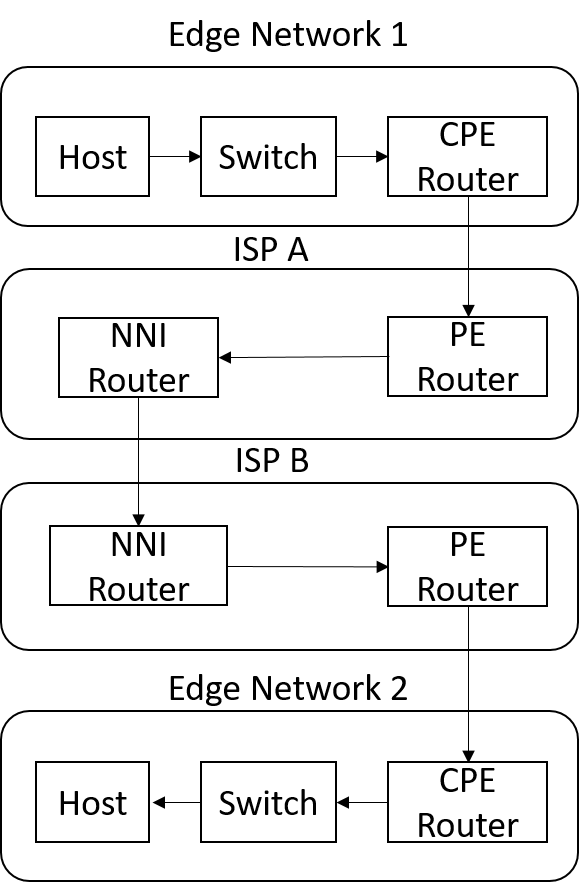
\includegraphics[width=5.79cm, height=8.82cm]{figures/eliminating2}
	\end{center}
	\caption{This illustrates five locations a source address can be validated: Host to Switch, Switch to CPE, CPE to ISP PE, ISP NNI to ISP NNI and ISP PE to destination CPE}
	\label{figure_eliminating} 
\end{figure}

For ISP Premise Edge routers, RFC 2827 \cite{rfc2827} encourages ISP's to use ingress filtering. This is as simple as the router checking if the source IP of a packet coming from a machine residing in, for example, \texttt{204.32.123.0/24} actually falls in this range. If it does not, the packet is discarded and the suspicious behavior is logged.

An advantage of this is that the origin of malicious datagrams can be determined and responsibility assigned. However, implementing such a technique is a widespread, collaborative solution to solving IP spoofing. This must be used everywhere for it to be effective. For example, the ISP might include an agreement in its service contract to use this procedure in its supplied router.

%%%%%%%%%%%%%%%%%%%%%%%%%%%%%%%%%%%%%%%%%%%%%%%%%%%%%%%%%%%%%%%%%%%%%%
\subsection{IP Source Guard \cite{ipsourceguard}}

Another router level implementation, this feature attempted to become a best current practice for defeating denial-of-service attacks in a switched LAN environment. It provides protection by limiting specific port access to clients that have received an IP address from the DHCP server (a standard network protocol to dynamically distribute IP addresses), rendering packet spoofing within the network impossible. 

However, the problem with implementing this on a router interface, is that illegitimate data will simply be discarded without advising the network or the user. Additionally, it is perfectly legal for a host to have more than one IP address. It is entirely possible that datagrams are sent using an IP address different from the interface's primary one. This would get discarded by the router and no error message returned.

This solution, although very effective, would only work for IP packets being spoofed as ones coming from inside the local network. This eliminates any local IP address authentication systems, but does not stop spoofed packets coming from outside the network.

%%%%%%%%%%%%%%%%%%%%%%%%%%%%%%%%%%%%%%%%%%%%%%%%%%%%%%%%%%%%%%%%%%%%%%
\subsection{Encoding Route Information Into Packets \cite{traceback}}
For practical deployment of IP traceback techniques, it was suggested that the IP identification field of IPV4 headers (primarily used for uniquely identifying groups of fragments of a single IP datagram, a practice that is not often used) could be overloaded to encode edge fragments. This meant that victims of IP spoofing could identify the network path traversed by the packets without requiring interactive suppose from the ISP.

Although promising work, RFC 6864 has since updated the IPV4 specification in 2013 to strictly forbid using the Identification field for any other purpose than what it was intended for \cite{rfc6864}.

%%%%%%%%%%%%%%%%%%%%%%%%%%%%%%%%%%%%%%%%%%%%%%%%%%%%%%%%%%%%%%%%%%%%%%
\subsection{Detecting Spoofed Packets \cite{dsp}}

Motivated by the messy variety and lack of an industry standard solution to the IP spoofing problem, S. J. Templeton and K. E. Levitt published a paper in 2003 discussing the attacks and various methods of detecting spoofed packets. They provided both active and passive approaches, as well as presenting results of experiments to verify the effectiveness of passive methods. 

Most notably, passive TTL methods were explored, based on the same assumption in this paper. The intuition for the approach was much the same, that packets coming from the same source should have similar TTL values, and if an anomalous packet is observed, then it may well be spoofed. However, no method for predicting expected TTL values for previously unseen IP addresses was implemented.

IP data was collected over a 2 week period, with over 23,000 unique IP addresses recorded. Using Conditional Entropy as an indicator of how predictable a TTL value was for a given source address, their conclusions indicated that TTL values appear to be highly predictable and thus can be the basis for spoofed packet detection. Although the accuracy was never tested, it was proposed that it is a good indication and can be used in conjunction with other methods as a first line of defence.

The paper concluded that 'no current detection method is 100\% correct'. Yet this does not devalue their utility, improvement is better than nothing. With a combination of more than one defence can greatly increase the effectiveness of identifying spoofed packets.

%%%%%%%%%%%%%%%%%%%%%%%%%%%%%%%%%%%%%%%%%%%%%%%%%%%%%%%%%%%%%%%%%%%%%%
\subsection{Hop-Count Filtering \cite{hcf}} \label{hcf}
In this paper from 2003, the idea of using a packet's hop-count to distinguish if it's spoofed is first brought to light. The feasibility of identifying spoofed packets using hop-count is discussed in great depth. Not only this, but the team managed to implement a simple filter to correctly identify 90\% of spoofed traffic. This is a testament of how worthwhile it can be to explore methods of spoof detection using TTL.

However, this considerably high accuracy requires an accurate mapping between IP addresses and hop-count. Not only this, but they made no effort to prove how practical the method is to be deployed at a large scale, withstanding legitimate DoS attacks.

To deal with unseen addresses, IP's are aggregated into a tree form, where hosts are grouped according to first 24 bits. This also reduces the space required for an IP to hop-count mapping. Although, in order to keep the false-positives suitably low, the percentage of false-negatives rose to roughly \%15 when grouping IP's like this. Furthermore, this still requires a large enough sample size. So upon deployment, the system will not have enough information to determine statistically different hop-counts, and must be left to gather data for at least a few days (depending on how busy the server is).

By default, the tool stays in 'alert state', monitoring traffic and comparing hop-counts to expected values using the IP to hop-count table. Once a sufficient amount of spoofed traffic is detected, indicating a DoS attack, the tool then switches to 'action state', in which most spoofed traffic is dropped. The switching of states is to prevent false positives when traffic is operating at normal levels. Only when a large increase in (particularly spoofed) traffic is observed, the tool then actually drops packets.

One of the more relevant findings that this team made, was the regularity of hop-counts observed. The distribution closely resembles that of a Gaussian curve, with the largest common hop-count value totalling to roughly 10\% of the IP addresses. Such a distribution is essential for TTL based methods to be successful. However, as Internet routing has been improved and changed within the last 15 years, it is important that this spread of TTL values still holds true today.

Similarly, the team measured the stability of Internet routing paths. To filter spoofed traffic based on hop-counts, routing paths must not change by too much too often. Otherwise, legitimate traffic that has been subject to a routing change might be identified as fake. Thankfully, they observed that 95\% of Internet routing paths had fewer than five changes per day. This, however, highlights the need for a dynamic, routing  change aware system - to be able to distinguish a change of route from a spoofed source address.

To counteract changes in routes, whilst in 'alert' state, small shifts in hop-count are all treated as legitimate changes. This, however, puts the system at risk of slow pollution of the IP to hop-count table whereby spoofed traffic is introduced slow enough as to not put the system into action state.

%%%%%%%%%%%%%%%%%%%%%%%%%%%%%%%%%%%%%%%%%%%%%%%%%%%%%%%%%%%%%%%%%%%%%%

\section{Limitations}
Although a low-cost, passive approach to the IP spoofing problem, solely relying on the TTL field in packet headers is not a definitive technique for identifying spoofed source addresses. This method theoretically cannot have 100\% detection rate for the reasons outlined below.

\subsection{Similar Location or Routes} \label{same_routes}
If the source address is faked to be one close by, perhaps the same sub network, then the TTL will be roughly the same and may not be statistically different enough to be classed as taking a different route to arrive. This is also the case if the faked source would take a similar amount of hops to the server than the attacker's packet would. Unfortunately, this would be impossible to detect looking at TTL alone.

However, being on the same sub network might raise suspicion as large streams of data would either be, depending on the attack, contained within the network or entering and exiting the network simultaneously. This could be picked up and action could be taken by a separate mechanism.

\subsection{Faking TTL Values}
Of course, like the source address, TTL fields can be set to whatever the sender chooses it to be. However, to fake a TTL to mimic that of what the spoofed source's would look like, the attacker must know or make very advanced approximations to the route taken from the fake source to the victim. This is a very hard, if not impossible, task to accomplish. And seeing as many attacks using IP spoofing use a wide array of spoofed addresses throughout their packets, this must be calculated for every spoofed address. An attacker aware of the use of TTL based detection systems cannot do anything about it. They must get the precise number of hops for the packets to be accepted. This means randomising the TTL makes no difference.

\subsection{TTL Prediction for Unseen IPs}
It is not reasonable to assume the database will always contain a given source addresses. Therefore, generating an expected TTL value for a source address cannot solely rely on previous data from the same source. A mechanism to predict TTL values for unseen addresses is desirable. For starters, the tool could only look at the first 24 bits of the address, allocated for the network prefix. The last 8 bits are reserved for host addressing, so we can assume that all IP addresses that only vary by these 8 bits are physically very close together, so TTL values will be very much the same. Furthermore, it might be possible to extend this assumption to a larger bit mask of 16. This theory can only be validated once the data collection tool has been built with sufficient data collected and analysed.

An engineering approach to this problem would be the aforementioned naive ping implementation. This consists of simply sending an echo request to the supposed source IP address and comparing the TTL values of the response with the one in the considered packet. This is certainly an effective way to deal with previously unseen IP addresses. Although time consuming, it only must be executed once on each new address. Subsequent requests from the same source will not be hindered by this check.

However, denial-of-service attacks that use IP spoofing typically choose fake source addresses at random from the entire IP address space. A side affect of this is that many of generated addresses will be unreachable. IP packets with such addresses are known as 'bogons'. These typically include: ones that are not in the range of allocated addresses by the Internet Assigned Numbers Authority (IANA), ones not delagated by regional Internet Registry that are allowed for public Internet use, or addresses privately reserved \cite{rfc1918}. Trying to calculate an expected TTL for such an address by sending an echo packet is impossible, as the request will never reach the machine, thus wasting time.

Standard DoS protection tools can detect if an IP address is unreachable and can categorise it as spoofed. This means bogon filtering can be used in conjunction with this method to prevent trying to calculate TTLs for unreachable addresses. However, to work around bogon filtering, more sophisticated spoofing tools avoid unreachable addresses. Thankfully, this increases the chance that the spoofed source has been observed before.

%The hop-count, or distance from a client to a server can change as a result of relocation of networks, routing instability, or temporary network failures. Some of these events are transient, but changes in hop-count due to permanent events need to be captured.
\subsection{Long Term Route Changes} \label{modes}
Unfortunately, routing across the Internet is never permanent. The TTL from a given client can shift due to temporary network failures, routing uncertainty or a physical relocation of networks. The system must be able to distinguish a routing change from the same IP and one from a completely different source (i.e. a spoofed packet). 

To combat this, the tool can consist of two different states. The concept, first described in section \ref{hcf}, has the spoof detection tool sit in a passive state, in which suspicious packets are noted as being significant but no action is taken upon them. Once the tool detects a considerable number of suspicious packets, indicating an attack, the tool switches to an active mode in which all packets that do not have the expected hop-count are discarded. This will not directly decrease the false positive rate of the detection system, but will vastly decrease the chances of action taken on false positives.

In the passive state, changes in TTL, whilst flagging the detection system as a routing change, will not have action taken upon them and so will be treated at legitimate changes in routing. This makes the system sensitive to permanent routing changes.

%%%%%%%%%%%%%%%%%%%%%%%%%%%%%%%%%%%%%%%%%%%%%%%%%%%%%%%%%%%%%%%%%%%%%%%%%%%%%%

% include specification
\section{System Design Overview}
Above all, the tool must be capable of handling large quantities of packets at high speeds. The very foundation of a DoS attack is sending huge amounts of traffic to overwhelm the server. To achieve this, the handling of packets must be done using a kernel module - pieces of code that extend the functionality of the kernel without required a recompilation. This is because IP packets are initially handled in kernel space, and the transition to user space is very costly. However, accessing databases, along with a wide array of useful tools, are not available in kernel space. Therefore, the permanent storage and decisions taken upon each packet must be done in user space. 

For this reason, the system is compromised of two separate programs running in parallel, with a single line of communication: a data collection kernel module and a spoof detection and reaction program. To reduce the impact of the delay introduced from transferring data from kernel space into user space, the logged packets will be aggregated and sent into user space in big chunks at regular, user defined time intervals.

From user space, there must be permanent storage for the logged IP addresses and corresponding TTLs. The obvious choice here is a database. This is discussed in further detail in section \ref{database}

With the end goal of being deployable onto a real server, it must be ensured that the tool causes no interference with normal operations. This not only includes making sure to not deny any legitimate requests, but avoid any crashes or delay in response time caused by the tool. Therefore, all traffic will be mirrored onto a monitoring or analysis machine, whereby the suspicious traffic is analysed and responses are sent to the main machine. Copying traffic to the analysis machine can be achieved easily by initialising a 'mirror port' on the main machine. This is a standard mechanism which directly copies all packets seen on one port to another port.

For the analysis machine to accept traffic that wasn't destined to it, \textit{promiscuous mode} must be enabled on the relevant network interface controller. This is a standard feature that causes all traffic to be sent to the CPU rather than just the packets the controller is programmed to accept. Then, for the packets to be passed through the network stack and analysed by the kernel module, the destination MAC address of the packets must equal that of the analysis machine. A simple program running on the main machine can easily change this as they are being mirrored.

\begin{figure}[h]
	\begin{center}
		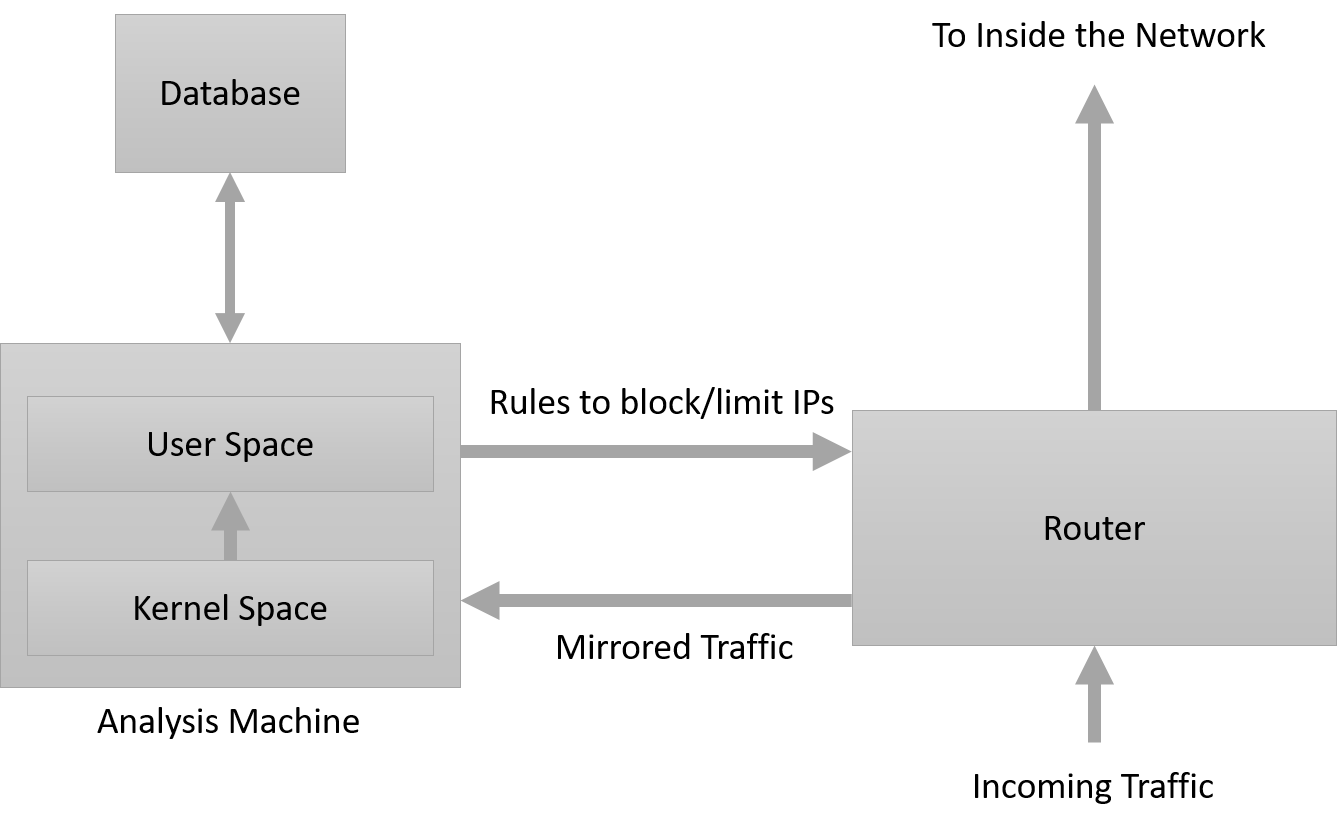
\includegraphics[width=13.4cm, height=8.31cm]{figures/system_layout.png}
	\end{center}
	\caption{The addition of TTL analysis will not hinder normal performance.}
	\label{figure_sys_layout} 
\end{figure}

Lastly, seeing as there is much more in depth work to be done on accurately classifying spoofed packets, work that cannot be achieved in this time frame, the tool must be easily extensible to allow for further development. Data gathered using this tool can aid in the additional analysis of determining spoofed packets. 

\section{Data Collection Tool} \label{kernel_tool}

Straightforward approaches to log traffic are available, for example iptables \cite{iptables}, a command line utility for configuring a Linux kernel firewall implementation. However, this is a large tool and struggles processing high volumes of data efficiently. Not only this, but extra data processing power must be wasted to aggregate the data into IP address and observed TTLs.

It would be much preferred to build a tool that more efficiently collects all incoming data, logs the useful information (source IP address and TTL) and store it in data structure, ready to be passed into user space when necessary.

%%%%%%%%%%%%%%%%%%%%%%%%%%%%%%%%%%%%%%%%%%%%%%%%%%%%%%%%%%%%%%%%%%%%%%
\subsection{Netfilter \cite{netfilter}}
Linux distributions provide a very useful packet filtering framework called Netfilter, allowing for fully customisable networking operations through the use of hooks. This enables kernel modules to register callback functions with the network stack. The function is then called for every packet that traverses the hook. One of the more popular features of Netfilter is the aforementioned iptables.

Netfilter libraries are shipped with all major Linux distributions, so the kernel tool should be able to run on a fresh install. However, the hook function has changed slightly numerous times throughout different kernel versions. To combat this, the code was made to be sensitive to whatever version the kernel is running on.

All of the Netfilter operations are done in kernel space, eliminating the need for costly translation of data between kernel and user space. However, developing and running in kernel space also has its disadvantages. For example: software bugs, such as memory errors, lead to kernel panics, requiring hard resets of the machine; some standard c functions are unavailable; and error messages and stack traces are difficult to interpret.

%%%%%%%%%%%%%%%%%%%%%%%%%%%%%%%%%%%%%%%%%%%%%%%%%%%%%%%%%%%%%%%%%%%%%%
\subsection{Utilising Threads}
To be capable of handling intense data loads, the time taken from receiving to accepting an IP packet must be minimised. If all operations to record the data were done on a single thread, then the process must wait for the data to be stored before it can let the packet through and start looking at the next one. Under high loads, this could result in packets being lost due to overflowing the available memory, either breaking the system or handicapping the capabilities of the program. Intuitively, concurrent execution must be utilised.

An initial strategy would be to simply start a kernel thread (kthread) in the netfilter hook callback function, passing the necessary data to be stored. However, the callback functions operate in interrupt context, and creating a kthread implicitly creates a thread scheduler that may sleep. Seeing as sleeping is strictly forbidden in interrupt context, this method will not work.

A neat solution to this problem are workqueues, a generic asynchronous execution mechanism \cite{workqueue}. Superficially, they allow kernel code to request that function be called at some time in the future. More importantly, adding work to a queue can be done in interrupt context so that it can be dealt with later, by another thread.

\begin{figure}[h]
	\begin{center}
		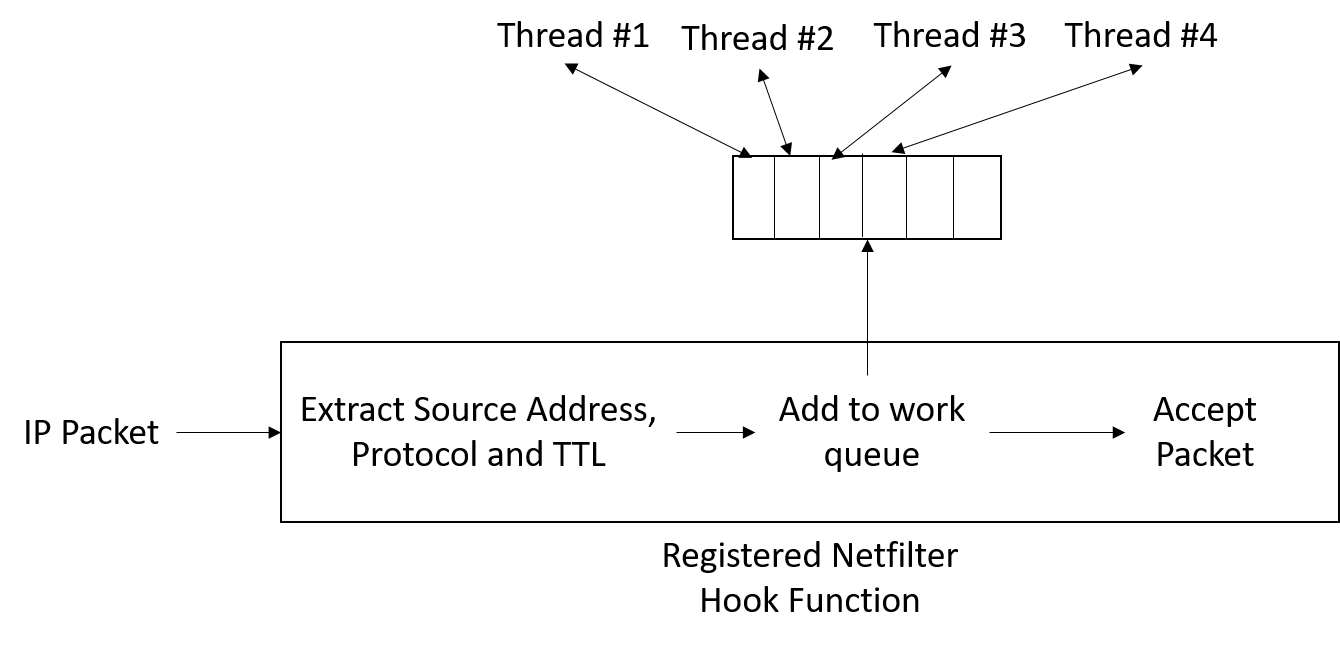
\includegraphics[width=7.37cm, height=3.55cm]{figures/workqueue}
	\end{center}
	\caption{Multiple threads take work out of the workqueue concurrently without delaying the packet flow}
	\label{figure_workqueue} 
\end{figure}

Most notably, it is possible to initialise a workqueue to have one dedicated kthread for each processor on the system. This further utilises all available computing power: not only can we separate the hooking from the processing of the data, but we can also separate the processing by having multiple threads taking work out of the workqueue and handling the data concurrently.

%%%%%%%%%%%%%%%%%%%%%%%%%%%%%%%%%%%%%%%%%%%%%%%%%%%%%%%%%%%%%%%%%%%%%%
\subsection{Efficient Data Structures} \label{data_structures}

Under high data loads, it is imperative to store the data as fast as possible. Even with multiple threads taking work out of the workqueue and processing it, the rate at which work enters the queue could be greater than the combined rate at which it's processed.

Storing data consists of two operations: lookup and insertion. In other words, we must first lookup the given source address in our data structure: if it exists, then we record the observed TTL value; if it does not, then we must insert a new data node to the structure. A sufficient data structure must be used to minimise these two costs whilst being practical to implement.

Initially, a linked list was implemented. However, for traversing the list, or lookup, this would take at most a number of operations equal to the length of the list. This is because each element must be looked at in order. Therefore, lookups take O(n) time - a time proportional to the number of items stored in the list.

A better approach is a binary search tree. The definition of this data structure requires that upon inserting a new node, it should be placed on one side of the tree based on some comparison - for IP addresses, this simply comparing the numerical address. To search or insert a given node, one must traverse, on average, nodes equal to the logarithm of the number of items stored in the tree. Therefore, lookup and insertion takes O(log n) time.

Other data structures were considered. For example a hash table. However, working in the limited memory of the kernel, a suitable hash function must be developed. And, seeing it was not possible at the time to know the distribution of addresses, an effective hash function is very difficult to create.

For the sake of efficiency, mostly motivated when performing comparisons in the search tree, IP addresses will be stored as an unsigned 32 bit integer in network byte order (the same form in which they arrive). There is no need to waste computing power by translating this into number and dot notation (e.g. \texttt{149.24.60.1}), as this would be stored as a character array which is considerably more costly to compare.

%%%%%%%%%%%%%%%%%%%%%%%%%%%%%%%%%%%%%%%%%%%%%%%%%%%%%%%%%%%%%%%%%%%%%%
\subsection{Multiple Writers Problem}

It was mentioned that it is efficient to utilise all processing power by have multiple threads taking work out of a workqueue and processing it concurrently. However, having multiple threads manipulating the same data structure introduces race conditions - behaviour dependent on the sequence or timing of uncontrollable events. For example, if two threads, t1 and t2, are traversing a binary search tree and trying to insert two different nodes, n1 and n2 respectively, perhaps they need to be inserted into the exact same position - say, the left child of n3. The execution order of the threads is undefined, so it could occur that both threads have traversed the tree and decided that the node needs to lie to the left of node n3, but have not yet inserted. When the threads go to insert their node, t1 could make the left child of n3 point to n1, and immediately after, t2 could also make the left child of n3 point to n2, overriding the previous assignment and completely losing n1, making it unreachable.. 

One solution is to initialise a mutual exclusion lock (mutex) that must be acquired before accessing the data structure. Only one thread at any given point can hold the lock, and a thread can only use the tree if it holds the lock. This ensures there is never a point where two or more threads are accessing the same data structure.

Although this eliminates all possible race conditions that might occur, it subsequently enforces a linear flow of execution amongst the threads. This is because the thread's only job is to traverse the tree and insert nodes, so mutex locks would ensure only one thread is executing at any time - completely invalidating any benefits of using threads.

\begin{figure}[h]
	\begin{center}
		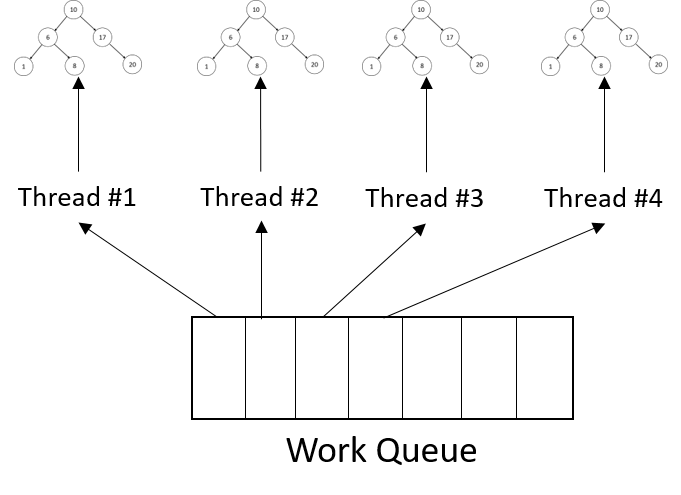
\includegraphics[height=5cm]{figures/trees}
	\end{center}
	\caption{Multiple threads working on multiple trees concurrently}
	\label{figure_trees} 
\end{figure}

A method is needed to enable multiple writers of data with no race conditions. To ensure this on the same, ever increasing data structure is a very difficult task. Instead, we can simply have multiple data structures. The solution chosen was to have work evenly distributed to multiple trees, so each thread can work on a different tree. This enables concurrency whilst preventing race conditions. A depiction of this can be seen in figure \ref{figure_trees}.

As we cannot guarantee which tree the data is inserted into, having multiple trees introduces the problem of duplicate entries for a source address. Although, implementing a mechanism to avoid this would require another data structure with checks, taking up valuable time. Because the data is only collected and inserted into the database every time interval, we can easily just sort out duplicate entries and aggregate the data at a later stage.


%%%%%%%%%%%%%%%%%%%%%%%%%%%%%%%%%%%%%%%%%%%%%%%%%%%%%%%%%%%%%%%%%%%%%%

\subsection{Testing and Evaluation}
The following evaluations were performed using an Intel i5-4200U CPU running at 1.6GHz with 4GB of RAM. These specifications are relatively low compared to some corporate machines, so expecting much better performance in the real world is entirely reasonable.

\subsubsection{Insertion Times}
Knowing an approximation of how long it would take to insert a node given the size of the tree data structure can be very advantageous. For example, it can be the case where the rate of incoming packets is greater than time taken for insertion given a tree size. If we can have a good estimate of the insertion time for a tree size, we can intelligently offload the data structure into user space when the tree becomes too big to handle the packet stream.

Being a binary search tree, the insertion time for a given node should be O(log \textit{n}) in the average case. To test this, 10,000 packets with unique source addresses were sent and handled by the kernel module and the time taken to insert it into the tree was noted. This was repeated 100 times and carried out twice: once with one tree, and once using a workqueue with four trees.

\begin{figure}[h]
	\centering
	\subfloat[One Tree]{{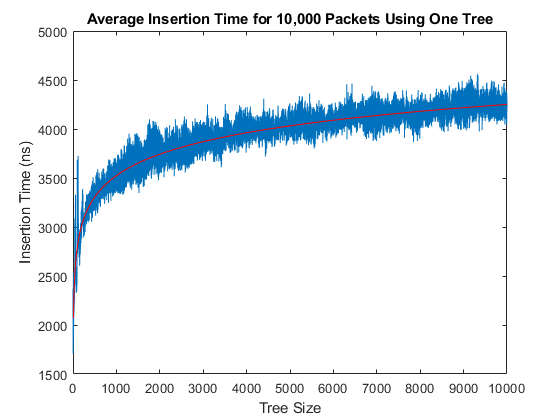
\includegraphics[width=7.7cm]{one_tree_fitted} }}
	\qquad
	\subfloat[Four Trees]{{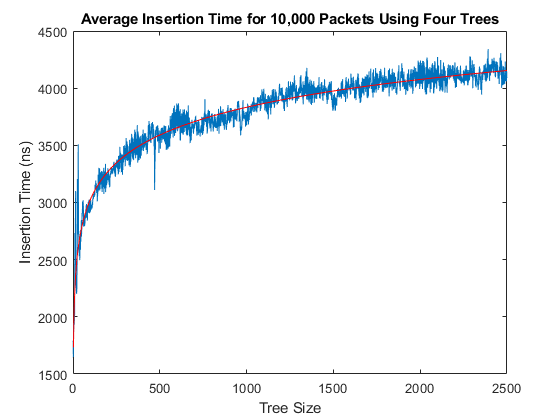
\includegraphics[width=7.7cm]{four_tree_fitted} }}
	\caption{Average insertion times for 10,000 packets.}
	\label{insertion_time}
\end{figure}

% Four tree: 1411 + 350.6 log(x)
% One tree: 1344 + 315.6 log(x)

Note that when using four trees, the packets are split evenly between them, meaning the maximum size of a tree was 2500, not 10,000.

Here we can easily fit a log curve onto the data. The fitted curve for one free was \texttt{1344 + 316 log(x)} and \texttt{1411 + 350 log(x)} for four trees. 

Now we can then determine a maximum packets per second for a given offload time. The maximum number of insertions for time t in nanoseconds, using one tree, is given by:

\begin{equation}
	\int_{x}^{0} 1344 + 316 log(x) dx
\end{equation}

Solving for x we find that

\begin{equation}
	 x = e^{W(\frac{t e^{\frac{257}{79}}}{316}) - \frac{257}{79}} 
\end{equation}
\\
Where W product logarithm function.\\
As an example, if the offload time was every second, a decimal approximation to the maximum number of packets the system could handle would be 204,415 per second. Using an average packet size of 557 bytes \cite{avg_pkt}, this is a theoretical maximum of 0.91 gigabits a second.

For a small network, a gigabit ethernet speed is common place. Although, for bigger networks, this can be easily exceeded in DDoS attacks. Therefore, better machinery  or split analysis would be required. 

\subsubsection{Effectiveness of a workqueue}
Theoretically, utilising threads seems worthwhile. Sending the work to be done by separate threads allows for more processing time for incoming packets. However, it could be the case that the computational power required to store all the data in a structure, initialise the work and send it to the workqueue could actually be greater than the time taken to store the data in the tree structure. 

Similarly, using four threads, simultaneously taking work out of the workqueue, requires synchronisation. Could simply using one thread be faster than four threads?

To test the effectiveness of using a workqueue and using four trees instead of one, 100,000 packets were sent in 0.1 seconds under these different conditions. The time taken to process all the packets was noted and this was repeated 100 times each.

\begin{center}
	\begin{tabular}{|c | c|} 
		\hline
		Version & Average Time Taken (Seconds)\\ [0.5ex] 
		\hline\hline
		No workqueue & 1.0215004\\
		\hline
		workqueue with 4 threads & 0.79763203 \\
		\hline
		workqueue with 1 thread & 0.83661073 \\ [1ex] 
		\hline
	\end{tabular}
\end{center}

Here we can see using a workqueue is beneficial, being roughly 20\% faster. Furthermore, we see that using four threads is 4.66\% faster than using only one. Although this is a small difference, it is still useful nonethless.

\subsubsection{Comparison with iptables}
The iptables utility, first written in 1998, has remained an integral part of network management in Linux operating systems. The code has stood the test of time, being trodden on, strained and seen numerous updates and rewrites over the years. This makes iptables an ideal benchmark to test the speed of data collection utility.

To test the speed of simply logging every packet seen (and in the case of the data collection tool, stored as well), 100,000 randomly spoofed packets were sent to the machine with a delay of 1 microsecond in between each one. The difference of time at which the first and last packet was logged were noted. On average, iptables took 1.742 seconds to log all packets, whilst the tool took 1.459 seconds. This makes the tool an average of 16\% faster than iptables.

\subsubsection{Limitations}
It was found that at roughly 250,000 unique IP addresses stored in kernel memory, the tool was unable to transfer this into user space. This was because the kernel memory allocation was simply too large and caused a devastating crash. To overcome this,  the traffic can be split between multiple analysis machines, or a mechanism could be built to transfer the data across in chunks of a set size. This, however, is a large engineering undertaking.

Even with this limitation, the number of unique IP addresses in between read times requires an impractically huge packet stream (even for that of a DoS attack). At peak times, one of the router computers in the University's Department of Computer Science would receive an average of 120 unique IP addresses every 60 seconds.

%%%%%%%%%%%%%%%%%%%%%%%%%%%%%%%%%%%%%%%%%%%%%%%%%%%%%%%%%%%%%%%%%%%%%%

\section{Spoof Detection Tool} \label{analysis_tool}

%It was accepted that the tool could not be made very accurate in terms of spoof detection given the lack of data analysis. Therefore, 
The main focus here lay on the engineering challenges introduced when developing a working, efficient spoof detection tool that was easily extensible. As a specification, the tool must do the following: acquire kernel data; make a decision based on this and all other past data; have a method to deal with previously unseen IP addresses; include a mechanism to block or limit future connections from the suspicious IP address; and be prepared and capable for future development. The tool was written almost entirely in C++ due to it's high performance and access to C functions required to read from the kernel module. 

To make the code extensible, a modular design pattern was adopted such that functionality is clearly separated and that extending the code only required a rewrite of either a small file or a single function. This was further made easier with C++ classes. Not only this, but the functionality of a module is easily changed by modifying a single value or switching to alternate functions that were written purely for customisability.

To deal with the first occurrence of an IP address, a small program was written in C. The code took heavy influence from the Ping utility included in all Linux distributions \cite{pingc}. The aim of this pinger program is to take in an IP address, send an ICMP echo packet and return the TTL of the reply packet. This is conclusive way of proving the correct TTL or hop-count for a given IP address.  

\subsection{Acquiring Kernel Data}
To transfer the data from the kernel module into the userspace process, Linux operating systems allow processes to be registered as pseudo files under the virtual file system \texttt{/proc/} \cite{proc}. These files usually contain runtime system information, but can also be treated as real files, allowing for other processes to execute read and write operations on them. Registered functions within the process handle the operations. In the case of the read function, the reader must supply a buffer, which is then filled with the required information by the registered process.

Upon a read request, the kernel module deconstructs all the internal tree structures, and fills up a buffer with each IP address and their corresponding observed TTLs and protocol. The most minimal representation is vital to save space. An example of this would be: \texttt{604346772u2x51 1x50t5x51}. The first number is the IP address in network byte order, whilst the characters 'u' and 't' indicate the start of the observed TTLs for protocols UDP and TCP respectively. This example depicts IP 604346772 having observed two occurrences of TTL 51 (2x51) and one of 50 for the UDP protocol; and five occurrences of TTL 51 for the TCP protocol. The space character is used as a delimiter for the list of observed TTLs.

\subsection{Pinger}
For the sake of modularity, an entirely separate program was written in C. This program contains a function that takes an IP address, sends an ICMP echo request packet to the address, waits for the reply and returns the TTL from the reply packet. 

The main concern when building the pinger utility was minimising the length of time wasted whilst waiting for the reply packet. Furthermore, it is entirely reasonable for a packet to be spoofed to an unreachable IP address, meaning there will never be a reply packet. Therefore, a time-out of 500ms was chosen for a maximum wait time for a reply. This number was chosen because the longest ping time measured was that of an Australian IP address taking 350ms. 

To reduce the time taken to ping a collection of IP addresses, a thread pool was utilised. Similar to a workqueue, this is where a group of pre-initialised threads wait for work to be passed through, each taking one piece of work. However, the simultaneous invocations of the pinger utility introduced interference problems. This is simply one instance receiving the wrong ICMP reply packet. To overcome this, a check was put in place that the source IP of the reply packet was the one in question. If not, the packet is ignored. Luckily, ignoring the packet does not discard it, but leaves it, ready for the next pinger instance to pick it up.

\subsection{Rule Manager}
The easiest way to limit or block IP addresses was to take advantage of the existing tool, iptables \cite{iptables}. However, the iptables functions are not externalised, and should never be used by developers as they could change any second \cite{iptablesapi}. The recommended method for using iptables in programs is to use the \textit{system\(\)} call.

A C++ class was created with functions to drop or limit IP addresses to a certain number of requests per second. The class held an internal list of active rules that dropped them after an allocated period of time to prevent clogging of the system. To allow for more fine-grained control, the functions for dropping packets could also specify a range of TTLs to accept.

Not all of the functions written were utilised in the spoof detector program. For example, a function to rate limit the provided IP address to a defined connections per second was created but never called. This is an example of making the code as extensible as possible, allowing for future development that has more intelligent and fine grained control of IP traffic. The functionality of class is well documented in the c++ header allowing for very strong customisability.

\subsection{Database Storage} \label{database}
The obvious choice to store large amounts of data in a permanent manor in user space would be a database. Initially, it was the case that the database would be stored locally to the machine to avoid costly connections to database servers. However, in the interest of making the data available to others without having to grant access to the analysis machine, it proved beneficial to add the option of using a database server rather than a local one. This not only allowed for simultaneous data analysis and spoof detection, but enabled a configuration whereby the traffic is split to multiple analysis machines to improve performance.

In the interest of efficiency and to preserve as much information as possible, the databases were set up such that each row consisted of the unsigned source IP address in network byte order as the primary key. Storing the address as a character array in numbers and dots notation decreased the speed of inserts by a considerable amount (roughly 10 times). This is because when using integers, the database system was able to create an index, which in turn creates a B-tree structure, making traversal O(log n). Furthermore, the convention for storing addresses on machines, known as host byte order, is dependant on the machine architecture. Therefore, the address is translated to the standardised network byte order whereby the most important byte is first (Big-endian) \cite{endianess}. The source address is then followed by 255 columns named TTL\_1 to TTL\_255 indicating the number of times the respective TTL was observed.

\subsubsection{SQLite \cite{sqlite}}
The well established and likely the world's most deployed database engine, SQLite, offers a self-contained and embedded database management system. Contained in a small C programming library, this is easy to implement with no configurations required.

SQLite uses simple database lock algorithms compared to more fine-grained ones found in other relational database managers, such as MySQL or PostgreSQL. Therefore, SQLite excels when there is only one user accessing it. This makes it much faster and more preferred if the database were to be stored locally. For these reasons, SQLite was chosen to be the database manager in development.

\subsubsection{PostgreSQL \cite{postresql}}
PostgreSQL is a reliable database manager with strong user management security. This is of great use when used as a database server with potentially sensitive information like a complete log of all client IP addresses. 

More importantly, PostgreSQL is installed as a database server. This means, with sufficient permissions, a user can remotely connect to the server and view/edit the database. Combined with strong database lock algorithms, unlike SQLite, it is possible to have multiple analysis machines updating the database concurrently. Therefore, if the speed penalty is sufficiently large, it can easily be distributed to multiple machines.

\subsubsection{Speed Comparison}
%Being the main constraint on this program, it was necessary to evaluate the speed of the two database managers. Packets were randomly generated, inserted and updated into the databases and the time taken to do so was measured. Results can be seen in figure \ref{sql_comp}.fa


\begin{figure}[h]
	\begin{center}
		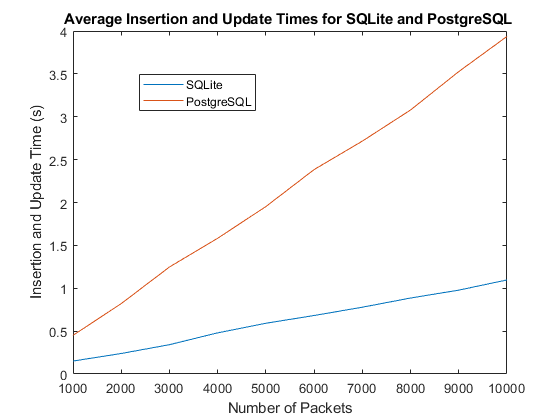
\includegraphics[width=10cm]{figures/sql_comparison}
	\end{center}
	\caption{SQL Database Manager Comparison}
	\label{sql_comp} 
\end{figure}

As expected, we can clearly see SQLite performing much more efficiently on a high number of insert/updates. Both managers follow a linear increase in time with respect to number of actions. This means that the time taken to bulk update can be easily predicted. In the case of using PostgreSQL, for a given input stream, we can calculate if the database update time is greater than the offload time interval. If it is, action can be taken - for example, initialise another analysis machine to split the load. For SQLite, a similar approach is difficult due to the local database with poor user management. 


\subsection{Testing and Evaluation}
Unlike the Kernel tool, evaluating success for the spoof detection tool is more of a discrete problem. Therefore, unit tests were written for some of the functionality and the results were compared with the desired output. This was the case for the rule manager and the pinger. Test code can be found in the git repository. 

In the case of database code, functionality was integrated into the tool, specific packets were sent under a test environment, and a database management interface was used to observe if everything was working correctly.

%%%%%%%%%%%%%%%%%%%%%%%%%%%%%%%%%%%%%%%%%%%%%%%%%%%%%%%%%%%%%%%

\section{IP Data Analysis} \label{analysis}
A port mirroring all traffic from one of the edge machines in the University of Birmingham School of Computer Science department was used to observe TTL values from over 5.7 million packets from 8570 unique IP addresses over a two week long period. It is worth noting that all packet payloads were discarded, preserving the data's integrity, meaning no ethical issues were raised.

This data was collected to calculate the distribution and predictability of TTLs. The values were converted to a probability of observation to avoid data skew from addresses seen more than others. This can be seen in figure \ref{ttl_count_prob}a. 

From the data, we can clearly observe three clusters, one at 40-50, one at 220-230, and a small cluster at 100-110. As described in section 1, this is due to the different initial TTLs used by protocols of 64, 128 and 255. From this, we can infer the initial TTL and calculate the hop-count. These are plotted again and can be seen in figure \ref{ttl_count_prob}b. 

\begin{figure}[h]
	\centering
	\subfloat[One Tree]{{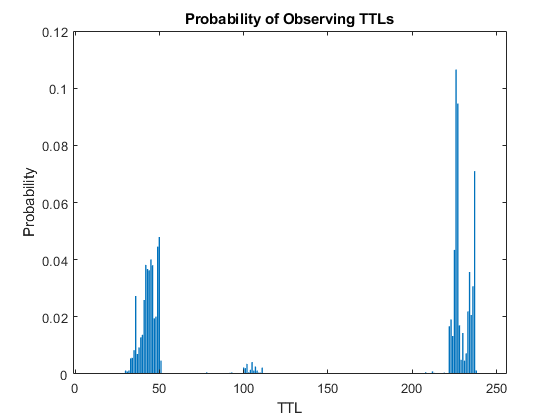
\includegraphics[width=7cm]{ttl_count_prob} }}
	\qquad
	\subfloat[Four Trees]{{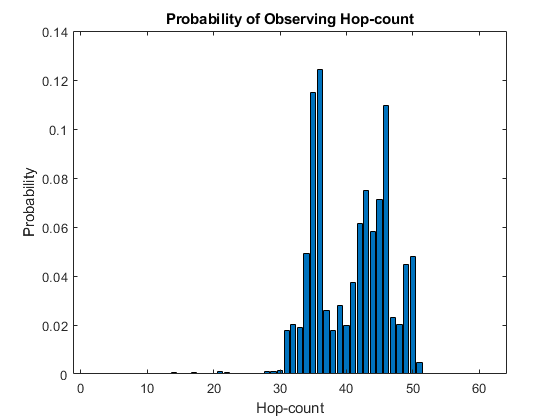
\includegraphics[width=7cm]{hop_count_prob} }}
	\caption{Average insertion times for 10,000 packets.}
	\label{ttl_count_prob}
\end{figure}

% 7.078%
\subsection{Distribution of TTLs}
Compared to the findings of the paper discussed in section \ref{hcf}, the hop-counts they observed followed a uniform Gaussian distribution. The same, however, cannot be said here.

As described in section \ref{same_routes}, one of the limitations with TTL analysis is if a spoofed packet just so happens to have the same TTL value as the expected one. With this distribution, we can calculate the probability of two random packets from separate sources having the same TTL. In this case, it is 7.08\%, making the theoretical accuracy of spoof detection 92.92\% when the system is in active mode (see section \ref{modes}).

However, it is worth noting that these distributions can vary depending on the type of traffic received. For example, a company that services the entirety of the UK with only one server will get a different distribution than a company with three severs placed at different locations. This is because requests will go to the closest server, so the company with one server will get a wider spread of TTLs. This has an effect on the accuracy of the method: the larger the spread of TTLs, the higher rate of detection the tool will have. The accuracy is given by:

\begin{equation}
	\sum_{i\in E}^{}P(x = i)^2
\end{equation}\\
Where E is the event set of all observed TTLs.

\subsection{Hop-Count Ranges}
To give an indication of how much the hop-count values vary with routing changes, the ranges of hop-counts were measured for the entire data sample. These ranges can be seen in figure \ref{ranges}. Here we can observe that 75\% of the observed hop-counts do not change at all. Of those addresses that do have varying hop-count values, 71\% of them only differ by one. 

\begin{figure}[h]
	\begin{center}
		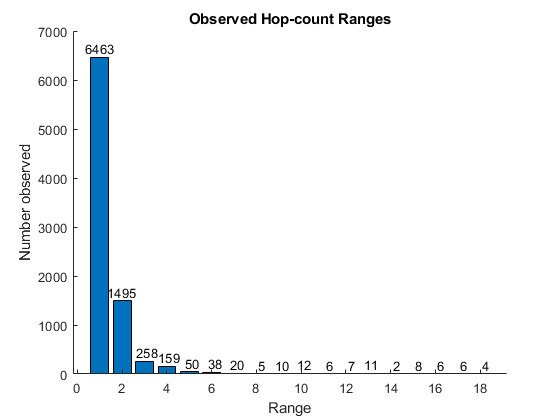
\includegraphics[width=10cm]{figures/hop_count_ranges}
	\end{center}
	\caption{Ranges of Hop-Counts}
	\label{ranges} 
\end{figure}
% global_variance: 0.450367
The calculated variance of hop-count for all IP addresses with more than one observed packet was 0.450. Knowing this, we can have further certainty to whether the received packet has a different hop-count due to either being spoofed, or a natural routing change. For example, even whilst in a passive state, if a packet is detected with a hop-count vastly different to what is expected, it can be discarded nevertheless. This would thwart all attempts in TCP hijack sessions (see section \ref{hijack}).

\section{Further Work}\label{future}
%Make it real time, more accurate detection, cluster IPs, use hash table, aging database
\subsection{Clustering IP addresses}
Pinging all first occurrences of an IP address, whilst a conclusive way of proving correct hop-count values, is a costly one. With further data collection and analysis, it could be possible to group IP addresses by hop-count values. Then, if patterns can be identified, (e.g. all addresses with 114.24.0.0/16 have a hop-count of 40), then TTL values from new IP address could be predicted.

\subsection{Kernel Data Structure}
The insertion time complexity of a binary search tree at O(log n), whilst very good, can still be improved. First mentioned in section \ref{data_structures}, a hash table could be a better alternative with an insertion complexity of O(1). However, due to the large chunk of memory dedicated to the hash table, the traversal of the entire table takes far longer than that of a binary search tree. Even though this is required only once per time interval, it is important that it does not take too long.

With the IP data collected, a suitable hashing function could be created in which IP addresses are evenly distributed through the hash table. However, this hashing function would have to change depending on the type of traffic received.

\subsection{Database Strategies}
The methods used for inserting and updating the databases were fairly naive. For SQLite, all observed IP's were attempted to be inserted into the database, and duplicate entries were ignored (using the SQLite keywords 'OR IGNORE', where upon inserting a duplicate entry, it is ignored instead of throwing an error). Then, updates were executed. For PostgreSQL, the database server was running version 9.2.23. This is of significance because below versions 9.3, the similar function, 'ON DUPLICATE DO NOTHING', was unavailable. In its place, a long winded workaround was required in which a temporary database was created and effectively merged with the current one.

Besides upgrading the PostreSQL version, we can further decrease the insertion time for both SQLite and PostgreSQL by utilising prepared statements. This is a feature used to execute similar statements with high efficiency. Although far trickier to implement due to the large number of columns, this should see a sizeable efficiency increase.

Furthermore, although the detection system is sensitive to permanent routing changes, this is not reflected in the database. The average hop-count from a given IP address in the database that has just been subject to a routing change will not be reflective of the true hop-count. To counteract this, the database could implement an ageing mechanism whereby the most recent observed TTLs influence the expected hop-count much more than old ones.

\subsection{Real Time Active Mode}
Currently, IP data is taken out of the kernel and processed in chunks at regular time intervals. For data collection, analysis and passive detection mode, this works sufficiently well. However, when switched to active mode, malicious packets are let through and only blocked after the data has been processed. Even if the decisions taken upon the packet on the analysis machine were real time, the packet would have still been let through due to the traffic being mirrored.

A better solution is that when the tool switches to active mode, the packets are picked up and checked real time \textit{on the router}. However, this not only introduces very difficult engineering challenges, but means the time taken to accept a packet in active mode is significantly increased. Whether this delay outweighs the damage caused by the malicious packets accepted in the previous method is a question that must be explored and tested.

\subsection{Route Change Analysis}
By monitoring certain Internet routes we can quantify how often routes change and by how much. Knowing this, we can build a characteristic of a route change and more intelligently recognise a natural alteration in hop-count, rather than identifying it as a suspicious packet. This kind of analysis requires route monitoring over a long period of time. For example, \texttt{traceroute} could be run on a set of IP addresses every regular time interval (10 minutes perhaps), and changes in routes can be observed. Regrettably, when this problem and analysis was considered, it was too late to start.

\section{Conclusion}
The goal of this project was to build an efficient system capable of identifying spoofed IP packets and taking action to block or limit further requests from the apparent source. The constructed tools were proved to be sufficiently fast at dealing with moderate to high data loads, but further development would be required to withstand large enterprise level DoS attacks. Furthermore, the effectiveness of certain design decisions in terms of speed were validated by running tests and analysing the results.

The system compromises of two tools: a kernel module to collect data, and a userspace program to detect spoofed traffic and deal with it. For storing the data, kernel side storage consists of binary search trees, whilst a database is used in userspace. Additionally, a mechanism to deal with previously unseen IP's was built and utilised, whereby an ICMP echo packet was sent to the IP address and the TTL of the reply packet was returned. To make it viable, this ping mechanism was implemented in an efficient manor using multithreading.

To vastly reduce the impact of false positives, particularly made relevant by natural routing changes, the system comprimises of two states: active and passive. By default, the tool sat in passive mode, in which no action is taken upon suspicious traffic. When the tool detects an influx of spoofed traffic, indicating a DoS attack, the tool switches to active mode, whereby all suspicious traffic is blocked.

The spoof detection tool was designed and built to be modular and easily extensible for further development. This was achieved with clear separation of functionality with highly customisable modules. The code is also usefully commented to make this process easier.

Finally, a large quantity of authentic IP traffic was collected and analysed to give further confirmation that a spoof detection approach using the TTL field in a datagram is sufficiently effective. In the active state, the tool would detect and block, on average, over 90\% of spoofed traffic. Even if the attacker is aware that TTL techniques were being employed, it would be too costly and difficult to overcome.

\section{References}
\bibliographystyle{asmems4}
\bibliography{reportBib}

\newpage
\section{Appendix}
\subsection{Zip File Submission Structure}
The submitted zip file is a compression of the 'tools' folder found in the project git repository link. This folder consists of three sub-folders: '\texttt{data\_collection\_tool}' where all the code for the kernel module is found; '\texttt{detection\_tool}' where all the code for the userspace spoof detection tool is found; and '\texttt{analysis\_and\_testing}' where all test files and data analysis results are found. The graphs displayed in this paper were generated using Matlab. The code used to generate the graphs is not contained, but the raw data is.

\subsection{Running the Code}
The contained code should be able to run on all major Linux distributions provided the relevant dependencies are installed.

\subsubsection{Data Collection Tool}
To compile the data collection kernel module, the relevant kernel source must be installed under \texttt{/lib/modules}. Then, run the \texttt{make} command in the \texttt{data\_collection\_tool} directory to create the kernel module files. Finally, execute the command \texttt{insmod firewall.ko} to insert the module. If successful, this should be represented in the kernel log file (often located in \texttt{/var/log/messages}).

\subsubsection{Spoof Detection Tool}
This tool requires the following dependencies to be installed: c++ version 11, \texttt{boost 1.66} c++ library, \texttt{libpqxx} for PostgreSQL functions and \texttt{sqlite3 libsqlite3-dev} library for SQLite functions. To utilise the PostreSQL functionality, the intended psql server credentials should be set in the psql.conf configuration file.

To compile the code, the \texttt{make} command should be run in the \texttt{detection\_tool} directory. The executable will then be generated. \textbf{Note, it is required that the program be run with root privileges.} To see the list of available arguments to the program, try running \texttt{sudo ./fwall\_reader -h}. A copy of this help menu can be found below:\\\\
\texttt{Usage: ./fwall\_reader\\
\tab 	-D\tab data collection mode - does not take action on suspicious packets\\
\tab 	-E\tab 	empties the kernel data structure but doesn't store the data\\
\tab 	-M\tab 	monitoring mode - logs TTL changes rather than dropping\\
\tab 	-P\tab 	uploads information to the psql database\\
\tab 	-p\tab 	{[}drop, accept, ping{]} first occurrence policy. (default accept)\\
\tab 	-R\tab 	cleans the database\\
\tab	-t\tab 	{[}time{]} time in seconds in between reads\\
}

\end{document}
